\documentclass{beamer}

\usetheme{Darmstadt}
\usepackage{listings}
\usepackage{xcolor}

\title[Compilation] {Compiling Software Packages}


\author[S.~Nakov] {Stojche Nakov}

\institute
{
  CS Departement\\
  Princeton University
}
\date[] {Group meeting, April 29, 2022}


\begin{document}

\frame{\titlepage}

\begin{frame}[fragile] \frametitle{Makefile project}
  \begin{columns}
    \begin{column}{0.5\textwidth}
      \begin{block}{Directory  structure}
        \includegraphics<1>[width=\textwidth]{dir_base}
        \includegraphics<2>[width=\textwidth]{dir_all}
        \includegraphics<3>[width=\textwidth]{dir_lib}
      \end{block}
      \uncover<2->{
        \begin{block}{make command}
          \centering
%%           \uncover<3>{:\$ make lib}
          \uncover<2->{:\$ make \only<2>{all}\only<3>{lib}}
        \end{block} 
        }
    \end{column}
    \begin{column}{0.5\textwidth}
      \begin{block}{Makefile} 
          \tiny{\begin{lstlisting}[language=make]
CC = gcc 
CFLAGS = -I include -g -Wall -O2
LIBS = -Llib -lmyLib
................
...............
all: $(TARGET)
lib: $(LIB)

$(TARGET): $(LIB) src/myExe.c
  $(CC) src/myExe.c  $(CFLAGS) $(LIBS) -o $@

$(LIB): $(OBJ)
  ar -rc $(LIB) $(OBJ)

obj/%.o: src/%.c
  $(CC) $(CFLAGS)  -c $< -o $@

$(DOC): doc/myLib.tex
  cd doc && pdflatex -pdf myLib.tex

clean:
  $(RM) $(OBJ) $(TARGET) 
  cd doc && pdflatex -c myLib.tex
            \end{lstlisting}
            }
      \end{block}
    \end{column}
  \end{columns}
\end{frame}

%% \begin{frame}[fragile] \frametitle{Makefile project}
%%   \begin{columns}
%%     \begin{column}{0.5\textwidth}
%%       \begin{block}{Directory  structure}
%%         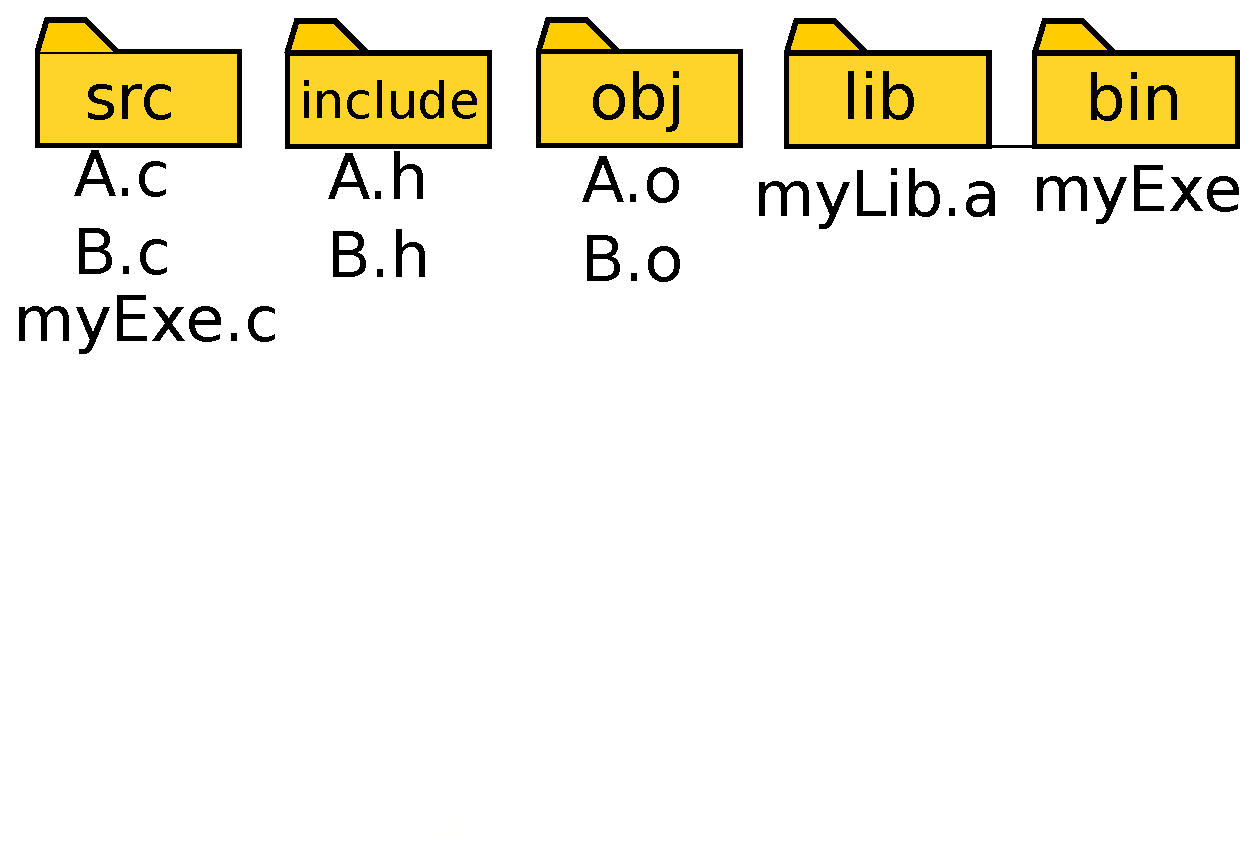
\includegraphics[width=\textwidth]{dir_all}
%%       \end{block}
%%         \begin{block}{make command}
%%           \centering
%%           :\$ make install
%%         \end{block} 
%%     \end{column}
%%     \begin{column}{0.5\textwidth}
%%       \begin{block}{Root directory} 
%%       \centering{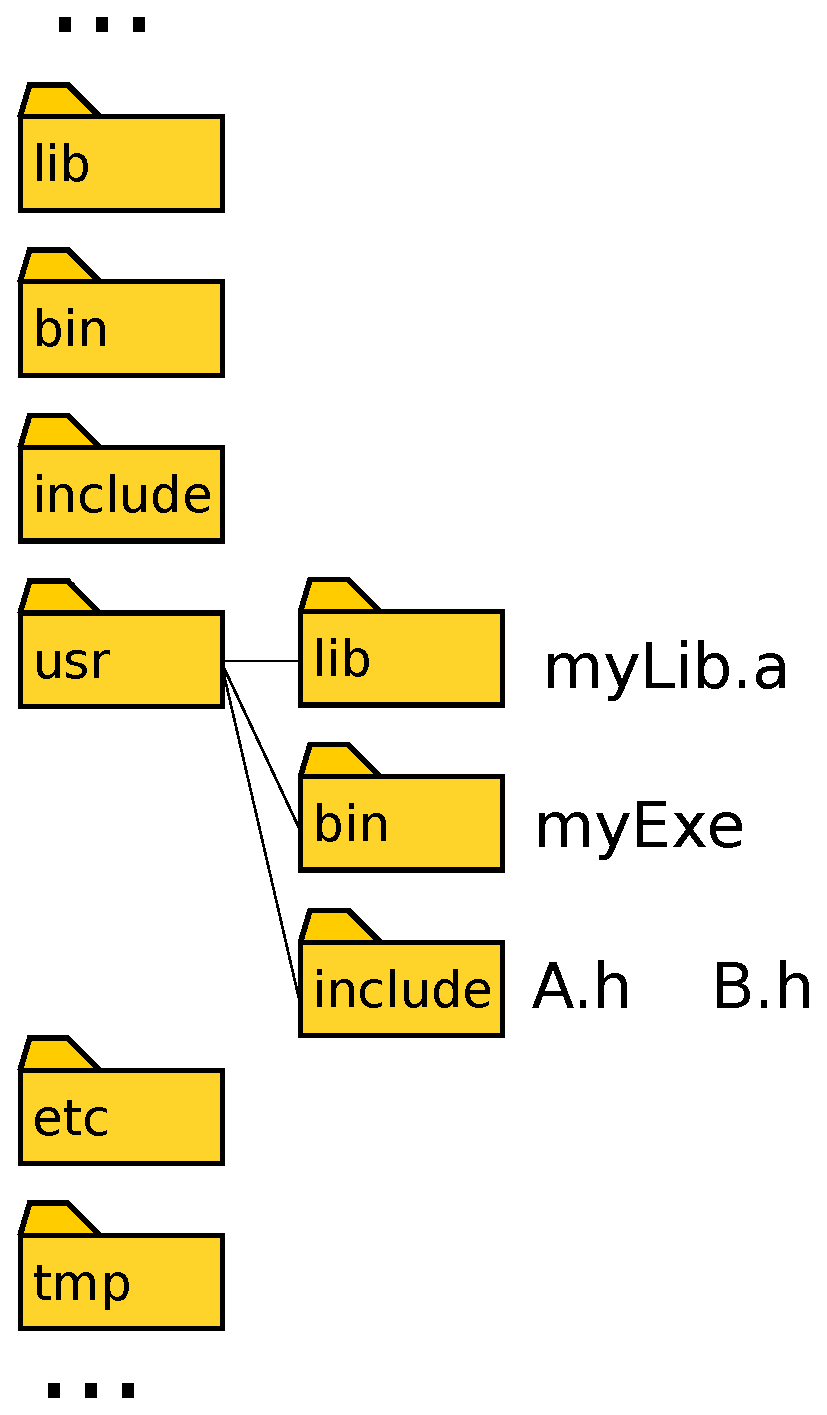
\includegraphics[width=.6\textwidth]{slash_dirs}}
%%       \end{block}
%%     \end{column}
%%   \end{columns}
%% \end{frame}


\begin{frame}[fragile] \frametitle{Makefile project}
  \begin{columns}
    \begin{column}{0.5\textwidth}
      \begin{block}{Directory  structure}
        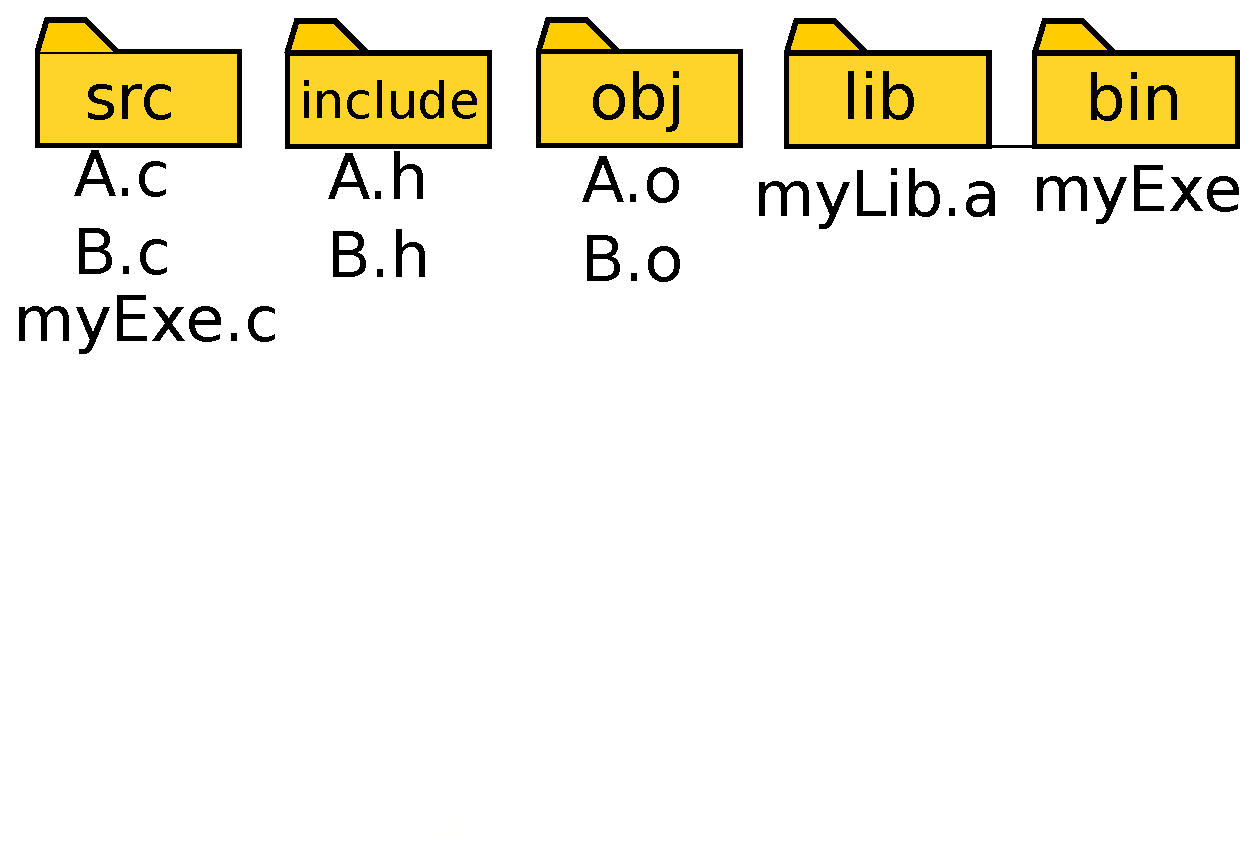
\includegraphics[width=\textwidth]{dir_all}
      \end{block}
        \begin{block}{Limitations:}
          \centering
          Platform  Portability 
        \end{block} 
    \end{column}
    \begin{column}{0.5\textwidth}
      \begin{block}{Makefile}
        \tiny{\begin{lstlisting}[language=make]
CC = gcc 
CFLAGS = -I include -g -Wall -O2
LIBS = -Llib -lmyLib
................
...............
all: $(TARGET)
lib: $(LIB)

$(TARGET): $(LIB) src/myExe.c
  $(CC) src/myExe.c  $(CFLAGS) $(LIBS) -o $@

$(LIB): $(OBJ)
  ar -rc $(LIB) $(OBJ)

obj/%.o: src/%.c
  $(CC) $(CFLAGS)  -c $< -o $@

$(DOC): doc/myLib.tex
  cd doc && pdflatex -pdf myLib.tex

clean:
  $(RM) $(OBJ) $(TARGET) 
  cd doc && pdflatex -c myLib.tex
            \end{lstlisting}
        }
      \end{block}
    \end{column}
  \end{columns}
\end{frame}

\begin{frame}[fragile] \frametitle{Makefile project}
  \begin{columns}
    \begin{column}{0.5\textwidth}
      \begin{block}{Directory  structure}
        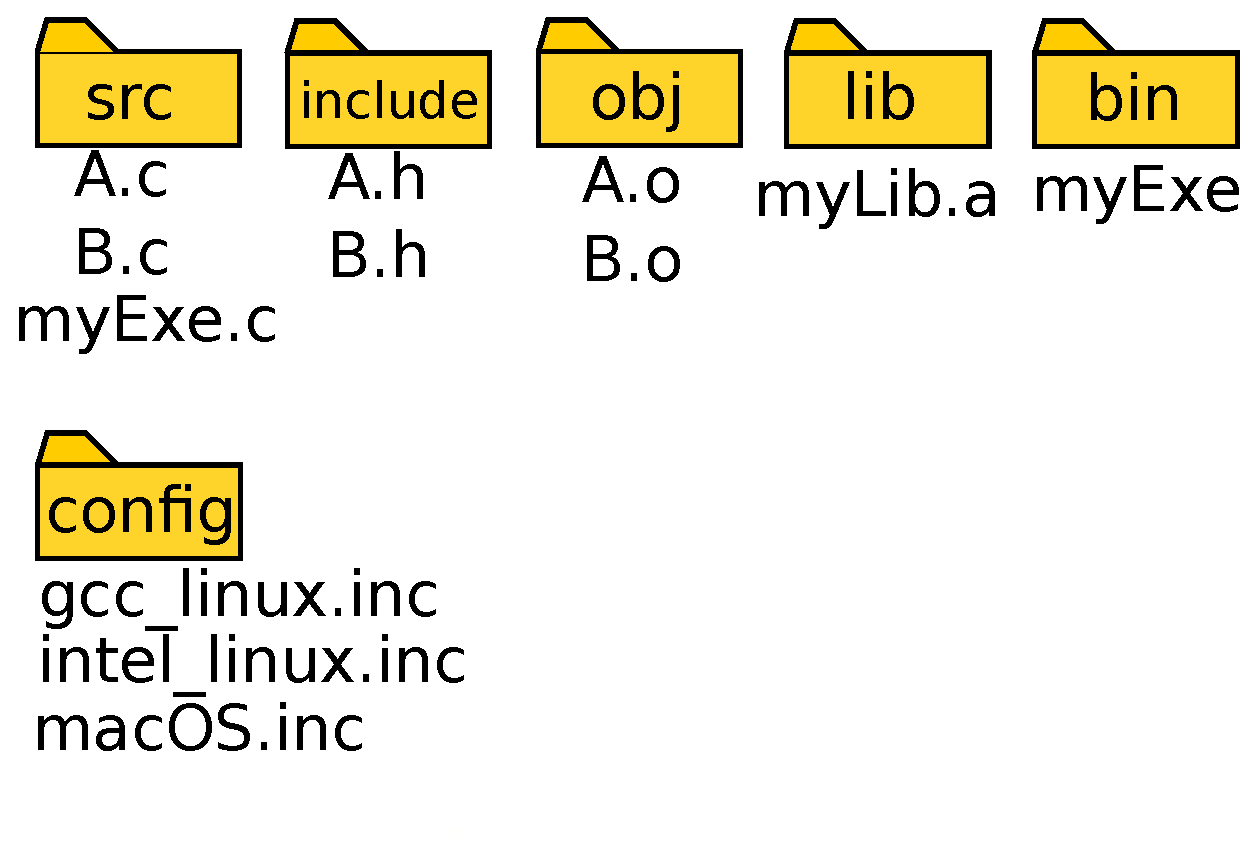
\includegraphics[width=\textwidth]{dir_config}
      \end{block}
        \begin{block}{make command}
          \centering
          :\$ make all
        \end{block} 
    \end{column}
    \begin{column}{0.5\textwidth}
      \begin{block}{Makefile}
        \tiny{\begin{lstlisting}[language=make]
include make.inc            
................
...............
all: $(TARGET)
lib: $(LIB)

$(TARGET): $(LIB) src/myExe.c
  $(CC) src/myExe.c  $(CFLAGS) $(LIBS) -o $@

$(LIB): $(OBJ)
  ar -rc $(LIB) $(OBJ)

obj/%.o: src/%.c
  $(CC) $(CFLAGS)  -c $< -o $@

$(DOC): doc/myLib.tex
  cd doc && pdflatex -pdf myLib.tex

clean:
  $(RM) $(OBJ) $(TARGET) 
  cd doc && pdflatex -c myLib.tex
            \end{lstlisting}
        }
      \end{block}
    \end{column}
  \end{columns}
\end{frame}

\begin{frame}[fragile] \frametitle{Autotools project}
  \begin{columns}
    \begin{column}{0.5\textwidth}
      \begin{block}{Directory  structure}
        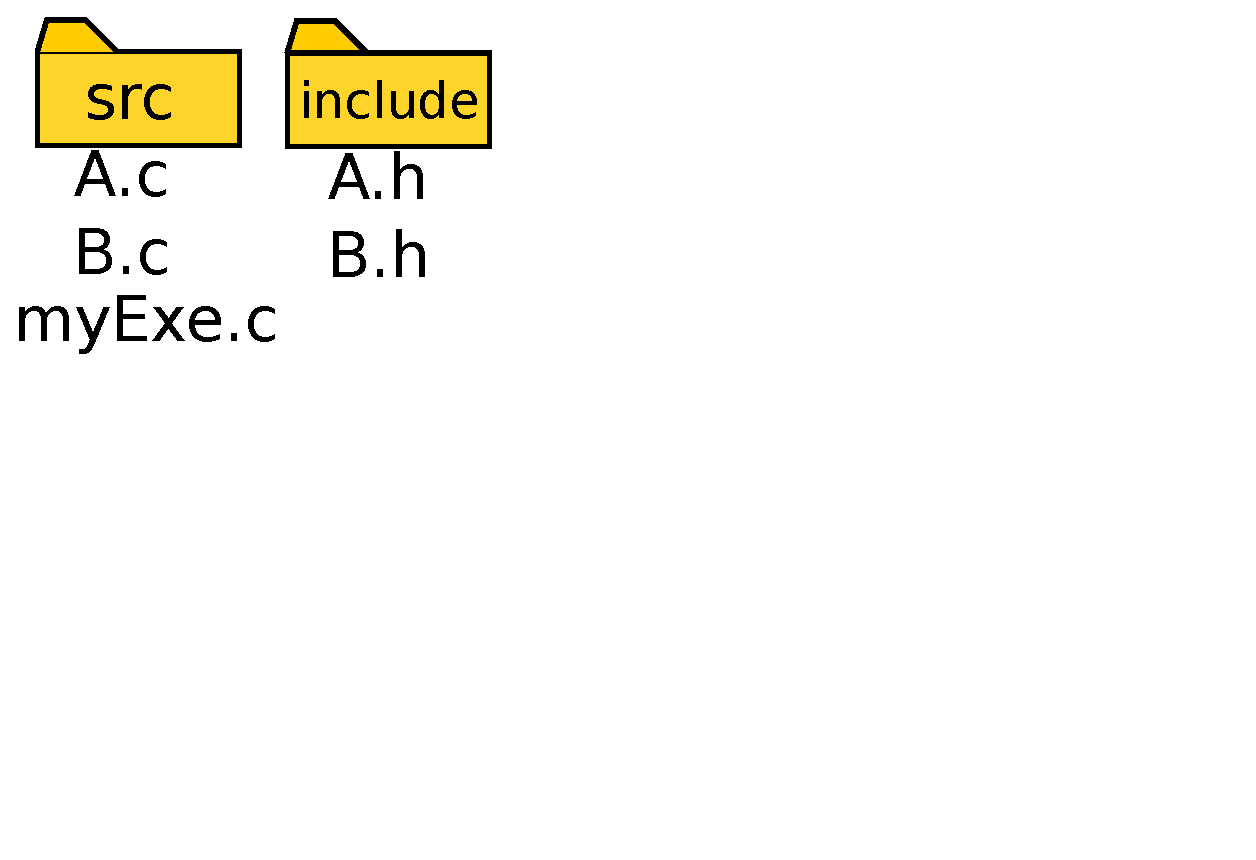
\includegraphics[width=\textwidth]{dir_cmake_base}
      \end{block}
    \end{column}
    \begin{column}{0.5\textwidth}
      \begin{block}{Autotools}
        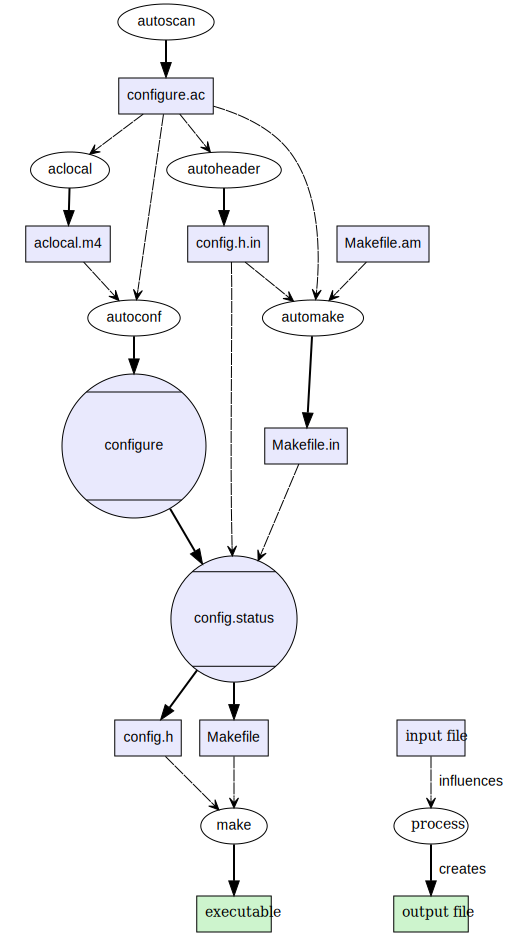
\includegraphics[width=.65\textwidth]{autotools}
      \end{block}
    \end{column}
  \end{columns}
\end{frame}

\begin{frame}[fragile] \frametitle{CMake project}
  \begin{columns}
    \begin{column}{0.5\textwidth}
      \begin{block}{Directory  structure}
        \includegraphics<1>[width=\textwidth]{dir_cmake_base}
        \includegraphics<2>[width=\textwidth]{dir_cmake_build}
        \includegraphics<3>[width=\textwidth]{dir_cmake_config}
        \includegraphics<4>[width=\textwidth]{dir_cmake_compiled}
      \end{block}
        \begin{block}{CMake commands}
          \centering
          \only<2>{:\$ mkdir build}
          \only<3>{:\$ cmake ..}
          \only<4>{:\$ make} 
        \end{block} 
    \end{column}
    \begin{column}{0.5\textwidth}
      \begin{block}{CMakeLists.txt}
        \tiny{\begin{lstlisting}[language=make]
cmake_minimum_required(VERSION 3.0)

project(Test_Project C) 

include_directories(include)

add_library(myLib src/A.c src/B.c)

add_executable(myExe src/myExe.c)
target_link_libraries(myExe myLib)
          \end{lstlisting}
        }
      \end{block}
    \end{column}
  \end{columns}
\end{frame}

\begin{frame}[fragile] \frametitle{Main Takeaways}
%%   \begin{columns}
%%     \begin{column}{0.5\textwidth}
%%       \begin{block}{Makefile}
%%         make \&\& make install
%%       \end{block}
      
      \begin{block}{Autotools}
        // Typical Autootls compilation  \\
        mkdir build \&\& cd build \&\& ../configure \&\& make  \\
        // Configuration: From the build directory \\
        ../configure --help 
      \end{block}
%%     \end{column}
%%     \begin{column}{0.5\textwidth}
      \begin{block}{CMake}
        // Typical CMake compilation  \\
        mkdir build \&\& cd build \&\& cmake .. \&\& make  \\
        // Configuration: From the build directory \\
        ccmake ..
      \end{block}
%%     \end{column}
%%   \end{columns}
\end{frame}
\end{document}
